% !TEX root = ../thesis-example.tex
%
\chapter{Methodology}
\label{sec:data}
\lipsum[1]

\section{This is a section}
\lipsum[2-4]

\begin{table}[tp!]
\caption{Training sample of false-positive planet candidates for the clustering algorithm.}
\tabcolsep=6.5pt %use this macro to add some regular space between lines (or squeeze it)
\hfill\begin{tabular}{l r r r l} 
 \hline
 \hline
 Star's identifier& 
\multicolumn{1}{c}{$T_{\mathrm{eff}}$} & 
\multicolumn{1}{c}{Lum} & 
\multicolumn{1}{l}{Luminosity} & 
Reference \\

 & 
\multicolumn{1}{c}{[K]} & 
\multicolumn{1}{c}{[L/L$_\odot$]} &  
\multicolumn{1}{c}{cluster}&  \\[0.5ex] 
 \hline
 $\pi$\,Her & 4170 & 1320 & High & \cite{Hatzes1999} \\ 
 $\mu$\,UMa & 3899 & 1150 & High & \cite{Lee2016} \\
 HD\,18438 & 3871 & 830 & High & \cite{Delgado2018} \\
 $\gamma$\,Dra (Eltanin) & 3990 & 510 & High & \cite{Hatzes2018} \\
 $\alpha$\,Tau (Aldebaran) & 4055 & 440 & High & \cite{Hatzes2015} \\ 
 \hline
 $\theta^1$\,Tau & 5000 & 70 & Low & \cite{Beck2015} \\
 NGC2423\,No.3 & 4592 & 65 & Low &\cite{Delgado2018} \\ 
 $\gamma$\,Psc & 4909 & 60 & Low & \cite{Beck2015} \\ 
 $\beta$\,Gem (Pollux) & 4865 & 40 & Low  & \cite{Delgado2018} \\
 IC4651\,No.9122 & 4720 & 35 & Low & \cite{Delgado2018} \\
 $\gamma$ Cep A & 4900 & 10 & Low & \cite{Hatzes1999} \\ 
 \hline
\end{tabular} \hfill~
\label{tab:false_positives}
% an empty line should be left between the tabular body and the table foot to avoid formating problems.

\tablefoot{The star's identifier is given. For the most prominent stars, the name of the star is amended in brackets.  The next columns report on the effective temperature and the luminosity of the star in units of the solar luminosity L$_\odot$. The typical uncertainty of the reported temperature and luminosity are 150K and $\sim$10\%, respectively. The top and bottom panel report classification of the clustering. The cluster name refers to the position in the red-giant phase. The literature references are provided in the last column. (Table taken from Elisabeth Höldrich bachelor thesis, 2020)}
\end{table}

\lipsum[4]

\subsection{This is a subsection}
\lipsum[4]

\section{Example of a code snippet \label{sec:MESA:Inlists}}
\lipsum[1]


\begin{table}[tp]
\begin{lstlisting}[language=Fortran,frame=Tb,
caption= Example for setting the tidal mechanisms in the \textit{star\_star} inlist. 
\label{code:tidalSettings}]{Name}
&binary_controls
	 do_tidal_circ = .true.
	 circ_type_1 = 'Hut_conv'
	 circ_type_2 = 'Hut_conv'
	 
	 do_tidal_sync = .false.
	 sync_type_1 = 'Hut_conv'
	 sync_type_2 = 'Hut_conv'
\end{lstlisting}
\tablefoot{A part of \textit{\&binary\_controls} environment in the \textit{star\_inlist} is shown.
The true/false-statements in line 2 and 6 determine if the models defined below takes into account the defined mechanism. 
The keywords for defining the formalistic description for circularization and synchronization mechanism are defined in lines 2-4 and 6-8, respectively. The number at the end of the keyword indicates which formalism is set for the primary (1) and secondary (2) stellar component.}
\end{table}


\lipsum[2-3]


\begin{figure}[pt!]
  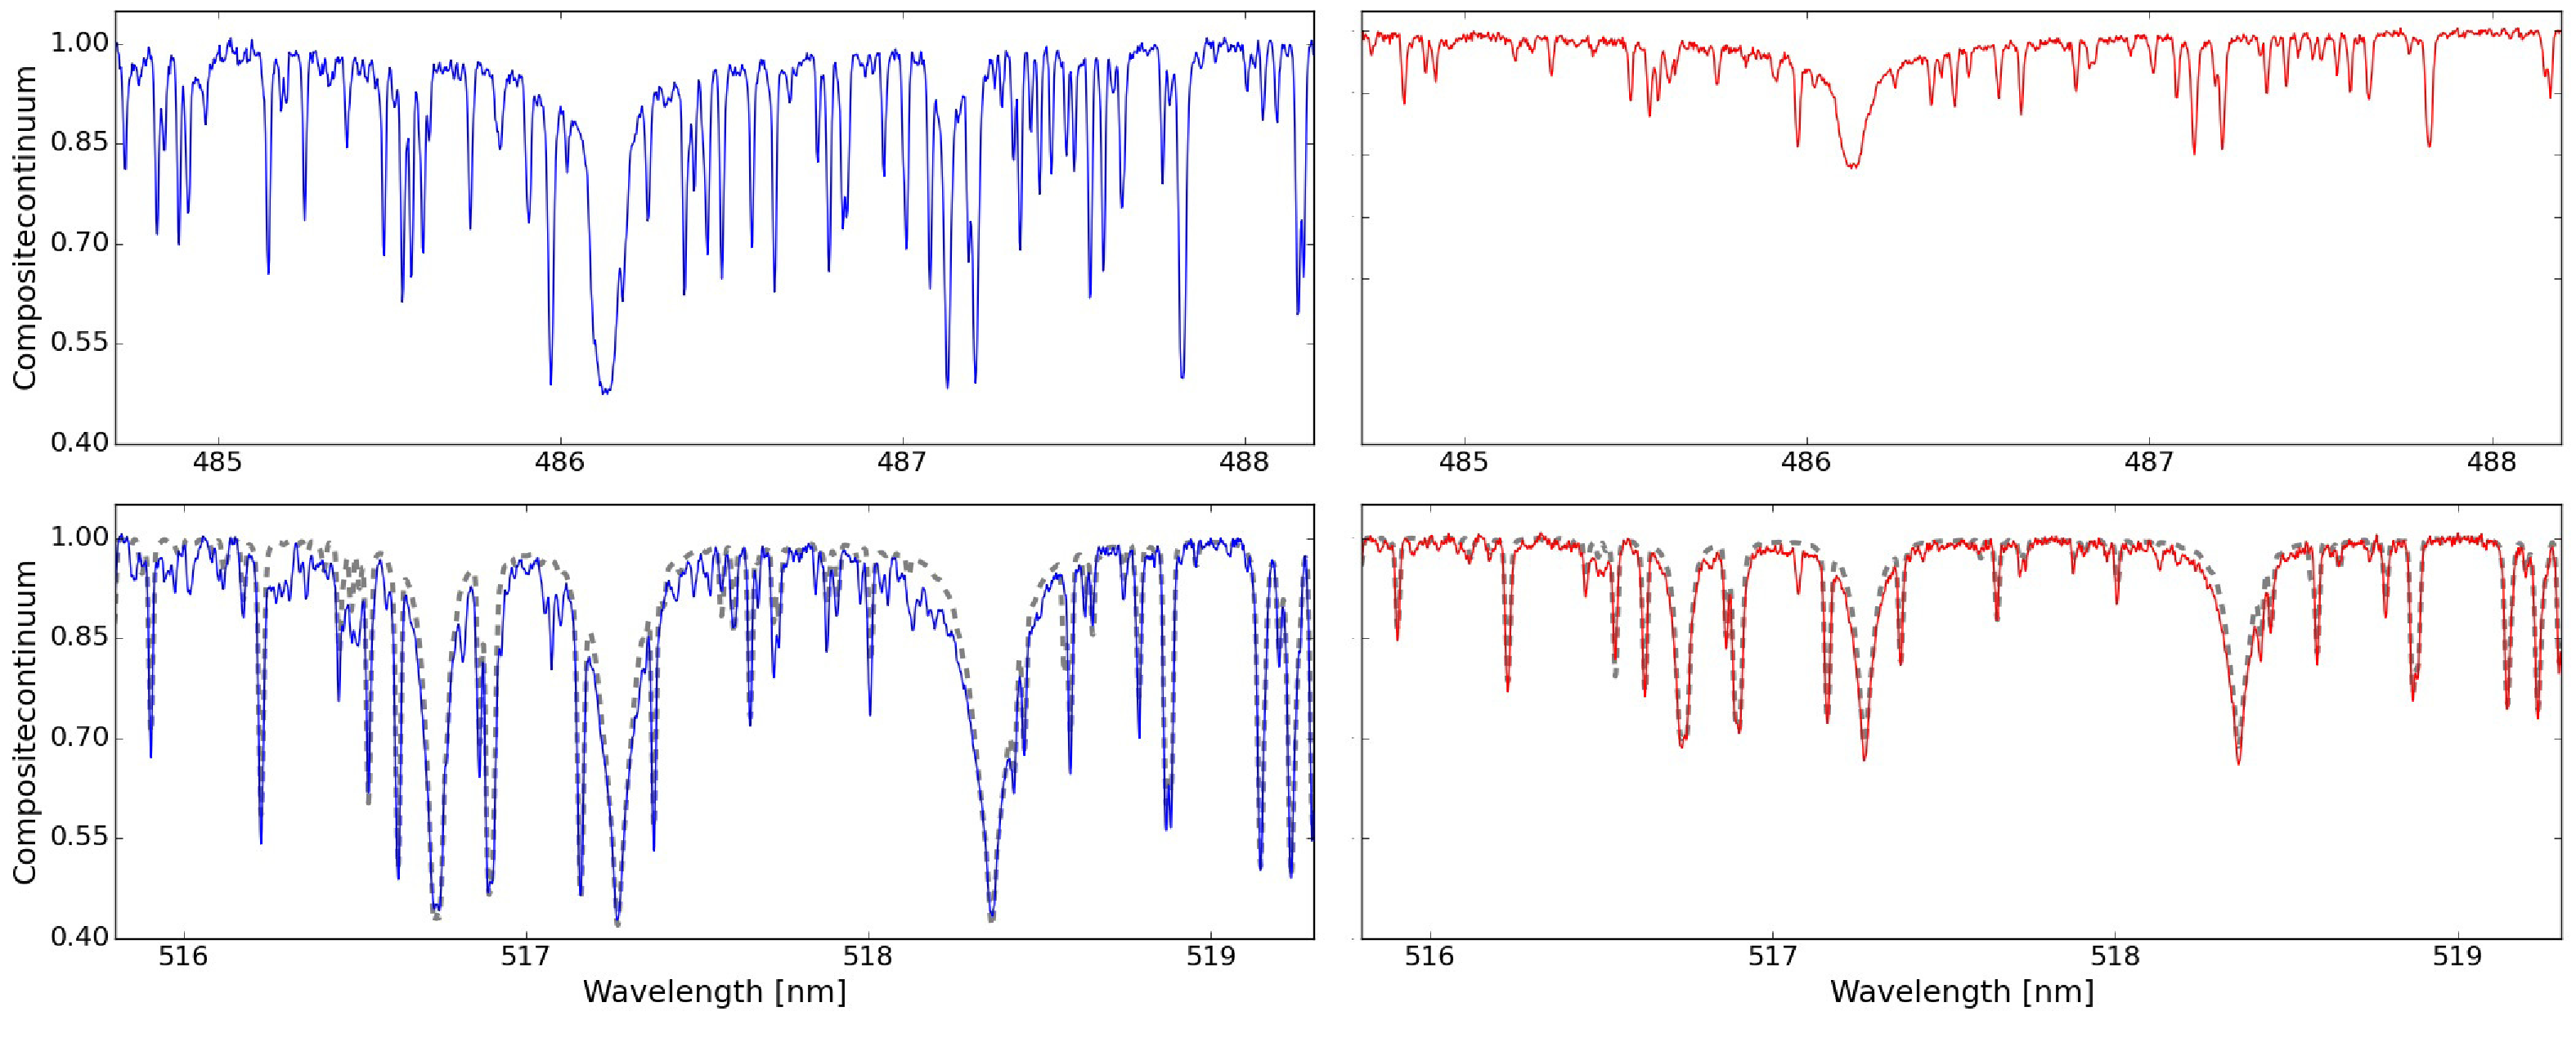
\includegraphics[width=\linewidth]{gfx/spectralSegmentDisentanlging.pdf}
  \caption{Disentangled spectra of KIC 9163796. The spectra of the primary in blue and secondary in red are shown in the left and right spectrum,
respectively. Top panel: the region around the H\textbeta line, while bottom panel: magnesium triplet at 518 nm, normalised to the continuum flux of the
composite spectrum. The synthetic model of the best fit of the determination of fundamental parameters and metallicity is shown as dashed grey
line is shown depicted in the region of the Mg triplet. \citep[Graphic taken from][]{Beck2018}}
  \label{fig:multiPanelPlot}
\end{figure}

\lipsum[3]


\begin{landscape}
\begin{table}[tp!]
\caption{
Seismic and fundamental parameters for 14 oscillating red giant heartbeat stars, ordered by descending orbital period.}
\tabcolsep=5pt
\hfill\begin{tabular}{c|rrrrrrrrrrrrrrrrrrr}
\hline \hline
\multicolumn{1}{c}{Star}  & \multicolumn{1}{c}{$\nu_{\mathrm{max}}$}  & 
\multicolumn{1}{c}{$\Delta\nu$}  & \multicolumn{1}{c}{$\Delta\Pi_1$}  & 
\multicolumn{1}{c}{$\delta f_{\mathrm{max}}$} &  \multicolumn{1}{c}{Evol.}  & 
\multicolumn{1}{c}{R}  & 
\multicolumn{1}{c}{M}  & 
\multicolumn{1}{c}{$\log g$} & 
\multicolumn{1}{c}{L}  & 
\multicolumn{1}{c}{T$_{\mathrm{eff}}$} & 
\multicolumn{1}{c}{$P_{\mathrm{orbit}}$} & 
\multicolumn{1}{c}{A}  & 
\multicolumn{1}{c}{$| \Delta $RV$|$} 	 \\
\multicolumn{1}{c}{KIC}  & 
\multicolumn{1}{c}{ [$\mu$Hz]} & 
\multicolumn{1}{c}{ [$\mu$Hz]} & 
\multicolumn{1}{c}{ [sec]} & 
\multicolumn{1}{c}{ [nHz]} & 
\multicolumn{1}{c}{Phase}  & 
\multicolumn{1}{c}{ [$R_\odot$]} & 
\multicolumn{1}{c}{ [$M_\odot$]} & 
\multicolumn{1}{c}{ [dex]} & 
\multicolumn{1}{c}{ [L$_\odot$]} & 
\multicolumn{1}{c}{ [K]} & 
\multicolumn{1}{c}{ [d]} & 
\multicolumn{1}{c}{ [ppt]} & 
\multicolumn{1}{c}{ [km\,s$^{-1}$]}
\\\hline

\hline
{9151763}	 & 13.8$\pm$0.2 & 1.98$\pm$0.01 	& $-$ & $-$ &  RGB? & 17.6$\pm$0.4 & 1.19$\pm$0.08 & 2.01 & 96$\pm$16 & 4290 & 437.5 & +7.1 & 32.2\\
{7431665}	 &54.0$\pm$0.7 & 5.46$\pm$0.02& $\sim$67 & $-$ &  RGB & 9.4$\pm$0.1 & 1.39$\pm$0.05 & 2.62 & 35$\pm$2 & 4580 & 281.4&-3.0 &[37.8]\\
{5039392} & 6.2$\pm$0.1 & 1.13$\pm$0.01 & $-$ & $-$ & RGB &  24.0$\pm$0.7 & 0.98$\pm$0.07 & 1.67 & 157$\pm$24 & 4110& 236.7 & -6.0 &42.3\\
{9540226}$^\star$ & 27.4$\pm$0.4 & 3.18$\pm$0.01 & $-$ & $-$ & RGB & 14.1$\pm$0.3 & 1.6$\pm$0.1 & 2.37 & 81$\pm$13 & 4600 & 175.4 &  -7 & 45.3\\
{8210370}	 &44.1$\pm$0.8 & 4.69$\pm$0.02	& $-$ & $-$ &  RGB? & 10.5$\pm$0.2 & 1.40$\pm$0.08 & 2.54 & 44$\pm$4  & 4585 & 153.5 & -5.3 & 22.1\\
{11044668}&50.2$\pm$0.2 & 5.65$\pm$0.01	& $\sim$60 & 83(?) &  RGB & 8.18$\pm$0.09 & 0.99$\pm$0.03 & 2.59 & 26$\pm$3 & 4565 & 139.5 & -3.8& [43.0]\\
{10614012$^\star$}&70.2$\pm$0.9	& 6.54$\pm$0.02 	& $-$ & $-$&  RGB & 8.6$\pm$0.2& 1.49$\pm$0.08 & 2.74 & 33$\pm$4 & 4715 & 132.1 & -4.7 &  49.3\\
{9163796}	 &153.2$\pm$0.7& 13.53$\pm$0.04	& $-$ & $-$&  RGB & 4.46$\pm$0.03 & 0.89$\pm$0.01 & 3.09 &  12$\pm$1  & 4820 & 121.3 &$\pm$0.5& 70.1 \\
{2444348} & 30.5$\pm$0.3& 3.26$\pm$0.01  	& $-$ & $-$ &  RGB & 14.9$\pm$0.3 &1.94$\pm$0.11 & 2.38 & 86$\pm$14 & 4565 & 103.5 & -1.7 & 7.7\\
\textbf{5006817}& 145.9$\pm$0.5 & 11.64$\pm$0.01 & 78 & 450 &  RGB & 5.84$\pm$0.09 & 1.49$\pm$0.06 & 3.08 & 19$\pm$3 & 5000 & 94.8 & -1.7& 23.5\\
8803882 & 347$\pm$3& 22.6$\pm$0.4& $-$ & 500(?) & RGB   & 3.68$\pm$0.1  & 1.4$\pm$0.1 & 3.45& 8$\pm$1& 5043 & 89.7 & +0.5 & [1.9]\\
{8144355}	 & 179$\pm$2& 13.95$\pm$0.04	& $\sim$78 & 210(?)&  RGB & 4.90$\pm$0.09 & 1.26$\pm$0.08 &3.16 & 12$\pm$2  & 4875& 80.6 & +2.1 & 18.9\\
{9408183} & 164.8$\pm$0.2& 13.29$\pm$0.02 & $\sim$93 & 450 &  RGB & 5.02$\pm$0.07 & 1.23$\pm$0.05 & 3.12 & 13$\pm$1  & 4900 & 49.7 & +1.5& 64.4\\
{2720096} & 110.1$\pm$0.7& 9.17$\pm$0.01 & $-$ & $-$ & RGB   & 6.98$\pm$0.08 & 1.54$\pm$0.06 & 2.95 & 23$\pm$2 & 4812 & 26.7 & +1.0& 4.0 \\
{8095275} & 69.3$\pm$0.3  & 6.81$\pm$0.01 & $-$ & $-$ & RGB & 7.78$\pm$0.08 & 1.21$\pm$0.05 & 2.74 & 25$\pm$3 & 4622 & 23.0 & -6.0 & 20.6 \\ 
 \hline
\end{tabular}\hfill~

\label{tab:asteroseismicValues}

\tablefoot{The star's identifier in the \textit{Kepler} Input Catalogue (KIC) is given. Eclipsing systems are marked  with an asterisk. The columns $\nu_{\mathrm{max}}$ and $\Delta\nu$ report the frequency of the oscillation power excess and the large frequency separation between radial modes for a given star. $\Delta\Pi_1$ quantifies the true period spacing of dipole modes. The maximum value of the detected rotational splitting $\delta f$ is listed. The evolutionary phase RGB describes H-shell burning red giant. Ambiguous values are marked with '?'. The columns $R$,\,$M$,\,$L$, and $\log g$ report the stellar radius, mass, luminosity, effective temperature and surface gravity from scaling relations, respectively. $T_{\mathrm{eff}}$ was adopted from the KIC. The uncertainties of $\log g$ are on the order of 0.01\,dex and for the temperature typically smaller than 150\,K. $P_{\mathrm{orbit}}$ gives the orbital period from photometry. The column $A$ lists the maximum amplitude of the heartbeat in a rebinned phase diagram. The error estimate for $P_{\mathrm{orbit}}$  and $A$ from the PDM is not reliable due to the remaining contamination of the solar-like oscillations and therefore not given. $|\Delta $RV$|$ reports the maximum difference in radial velocity. Squared brackets mark systems for which the orbital parameters could not yet be determined from radial velocities. \citep[Table taken from][]{Beck2014}}

\end{table}%
\end{landscape}

 
